\documentclass{article}
\usepackage[T1]{fontenc}
\usepackage{lmodern}
\usepackage{graphicx}
\usepackage{amsmath,amssymb}
\usepackage[a4paper,margin=2cm]{geometry}
\usepackage[absolute,overlay]{textpos}
\setlength{\TPHorizModule}{1mm}
\setlength{\TPVertModule}{1mm}
\usepackage[indonesian]{babel}
\usepackage{hyperref}
\setlength{\emergencystretch}{2em}
% unit: Halaman 15

\begin{document}

% === Halaman 15 (python/native) ===

15

• Pada mode ECB, blok plainteks yang sama selalu dienkripsi 

menjadi blok cipherteks yang sama.


• Pada contoh di atas, blok 1010 muncul dua kali dan selalu 

dienkripsi menjadi 0010.

% deskripsi: gambar native xref 84
\noindent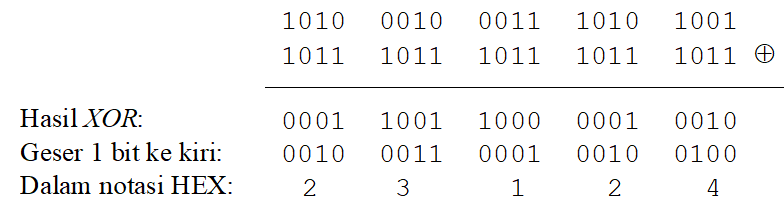
\includegraphics[width=0.85\textwidth]{../../images/python/page_015_img_01.png}

\end{document}
